\chapter{Metoder indenfor billedbehandling}\label{subsec:kant}
Formelt kan et gråtonebillede repræsenteres som en funktion af to variable:
\begin{equation}
\begin{split}
&I: \mathbb{\mathbb{Z^+}}^2 \rightarrow \mathbb{Z}^+ \\
&I(x,y) = \lambda_{x,y} \hspace{0.5 cm} (x,y)\in \mathbb{Z^+}^2, \lambda_{x,y} \in [1,256] \subset \mathbb{Z^+}
\end{split}
\label{bf}
\end{equation}
hvor $\lambda_{x,y}$ repræsentere en billedintensitet, også kaldet en pixelværdi. $\lambda_{x,y}$ er defineret, indenfor grænserne af billedet og er 0 udenfor, dvs.: 
\begin{equation}
 I(x, y) =
\begin{cases}
    \lambda_{x,y}, & \text{hvis } 1 \leq x \leq x_{max}, 1 \leq y \leq y_{max} \\
    0,              & \text{ellers}
    \label{pixelintensitet}
\end{cases}
\end{equation}
En kort bemærkning bør gøres om det anvendte billedformatet. De undersøgte billeder er af filtype JPEG(Joint Photographic Experts Group) og hver pixelintensitet indeholder originalt 8x3 bits information til hhv. rød, grøn og blå: $\Lambda_{x,y} = [R,G,B]^T \in \mathbb{R}^3$. Hver farve kan antage $2^8 = 256$ forskellige værdier og hver værdi ligger i intervallet $[0,1]$. Disse værdier bliver transformeret til en gråtoneværdi:
\begin{equation}
Lum(\Lambda_{x,y}) = \lceil	 256 \cdot [0.299, 0.587, 0.114] \Lambda_{x,y} \rfloor	 = \lambda_{x,y}
\label{lumosity}
\end{equation}  
Hver gang pixelværdi eller billedintensitet benævnes, er det underforstået, at de har undergået den lineære transformation, ligning \eqref{lumosity}. I denne opgave håndteres kun gråtonebilleder, derfor er ligning \eqref{lumosity} brugt til at transformere RGB billeder til gråtone billeder \footnote{I Python er biblioteket cv2 anvendt. Transformationen fra RGB til gråtone dokumenteret her %\url{<http://docs.opencv.org/2.4/modules/imgproc/doc/miscellaneous_transformations.html>}. 
Denne transformation bliver nærmere beskrevet i \cite{lumosity}. en uddybning og alternativer kan læses i afsnit 7.6} 
\\
\\
Ofte i billedbehandlings situationer betragtes diskontiniuteter i billedet, f.eks. kanter.
Hvis et billede beskues i 3D, kan en kant illustreres i 1D, ved et snit af et billede vinkelret på fladen i gradientens retning, illustreret i figur \ref{fig:kant}. En kant er en lokal ændring i det afledte signal $f$.
\noindent
\begin{figure}[H]
    \centering
    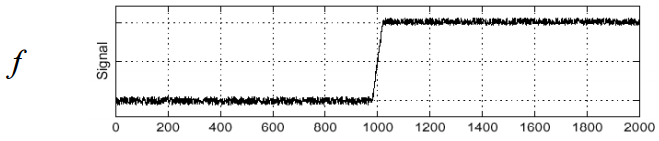
\includegraphics[width=0.55\textwidth]{fig/7.png}
     \vspace{-1em}
    \begin{center}        
     \caption{{\footnotesize \textit{
En 1-dimensional fortolkning af intensiteten i et billede. Intensitetsskiftet i midten (ved x $\approx$ 1000, er en kant.)}}}
    \label{fig:kant}
     \end{center}
       \vspace{-2.5em}
  \end{figure}
\noindent
En differentiering af funktionen fra figur \ref{fig:kant} en stigning i pixelintensiteten  og derved angive hvor der forekommer kanter. Differentiering af billeder kan f.eks. approsikmeres ved følgende ligning:
\begin{equation}
\dfrac{df(x)}{dx}=\dfrac{f(x+1)-f(x-1)}{2}
\label{diff}
\end{equation}
<ct Foldning er en operation, der indenfor billedbehandling bruges til modificere et billede. Modificeringen kan f.eks. være sløring, fokusering eller fremhævning af visse strukturer </ct>. Foldning af $I$ af størrelse $(M \times N)$, med en kerne $K$, der har størrelse $(k \times l)$, hvor $M > k, N > l$, angives ved:
\begin{equation}
O(i,j) = \sum_{k} \sum_{l} I(i-k, j-l) K(k,l)
\label{foldning}
\end{equation}
Ligning \eqref{foldning} udregnes for alle $i,j \in I$. En kerne defineres her som en matrix af arbitrær dimension - ofte $(N\times N)$. 
\\
\\
Et billede kan differentieres, som anført ligning \eqref{diff}, ved brug af foldning. Først defineres en kerne til differentiering i $x$-aksen $K$, som: $K = [\frac{1}{2}, 0, \frac{1}{2}]$. Kernen foldes med billedet $I$: $I \ast K $, hvor $\ast$ udgør foldningsoperatoren. Når en kerne skal foldes med et billede hvor afstanden til randen af billedet er skarpt mindre, end størrelsen af kernen, gælder ligning \eqref{pixelintensitet} for $I$.
\\
\\
Det kan være problematisk at lokalisere kanter vha. differentiering. I figur \ref{fig:kant}, vil støj i billedet(de små udsving) også blive fremhævet. For at fjerne støjen, kan billedet foldes med et Gaussisk filter, hvilket er en diskret approksimering til den Gaussiske funktion. Foldning af et billede med et Gaussisk filter vil resultere i en flydende overgang af pixelværdierne og derfor glatte billedet. <sæt gaussbillede ind> Den Gaussiske funktion i 2-D, hvor $ \sigma $ er standardafvigelsen af den Gaussiske fordelingen, er defineret som:
\begin{equation}
G(x,y,\sigma) = \frac{1}{2 \pi \sigma ^{2}} e^{- \frac{x^{2} + y^{2}}{2 \sigma ^{2}}}
\label{2dgaussian}
\end{equation} 
For at undgå først at glatte billedet ved at folde med et Gaussisk filter, og derefter folde med et differentieringsfilter udnyttes det, at foldning er en associativ operation:
\begin{equation}
\dfrac{\partial}{\partial x}(G \ast f) = (\dfrac{\partial}{\partial x}G) \ast f
\end{equation}
Her er $G$ er det Gaussiske filter, men kunne være en vilkårlig anden kerne, og $f$ et signal. 
\\
Foldes et differentieret 1-dimensionelt Gaussfilter med signalet fra figur \ref{fig:kant}, vil det resultere i et bakkeformet signal, hvor bakken indikere en kant \\ <ct billede /ct> \\ . For en mere lokaliserbar kant, kan den dobbelt afledte tages, som set i figur \ref{fig:deriv}. I sidstnævnte tilfælde, kan kanten lokaliseres, hvor funktionen krydser nul.
\begin{figure}[H]
    \centering
    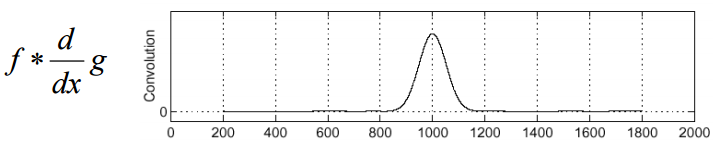
\includegraphics[width=0.55\textwidth]{fig/8.png}
    \vspace{-1em}   
    \begin{center}
    \caption{{\footnotesize \textit{
     Resultatet af at folde et dobbelt differentieret Gaussisk filter med funktionen}}}
    \label{fig:deriv}
     \end{center}
    \vspace{-2.5em}  
  \end{figure}
\noindent
I de anvendte metoder er der blevet gjort brug af et dataindsamlingsvindue. Med dette menes et udsnit af et billede, omkring et punkt. Figur \ref{fig:dataindvin} illustrerer et dataindsamlingsvindue omkring $I(3,4)$, der har størrelsen $(3 \times 3)$. Det skal bemærkes, at et dataindsamlingsvindue i denne opgave også kan bestå af andre værdier end pixelintensiteter. Det indeholder også gradient størrelse og gradient retninger.
\begin{figure}[H]
    \centering
    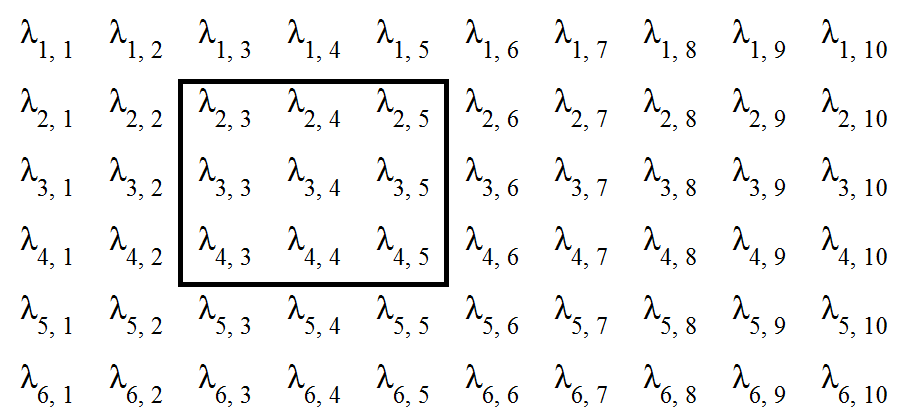
\includegraphics[width=0.55\textwidth]{fig/dataindsamlingsvinduepic.png}
    \vspace{-1em}   
    \begin{center}
    \caption{{\footnotesize \textit{
     Resultatet af at folde et dobbelt differentieret Gaussisk filter med funktionen}}}
    \label{fig:dataindvin}
     \end{center}
    \vspace{-2.5em}  
  \end{figure}
\noindent